\chapter[Referêncial Teórico]{Referêncial Teórico}

Neste capítulo serão abordados os temas relevantes para a compreensão teórica do trabalho proposto. O capítulo foi dividido em três seções, Teorias de Aprendizagem, Sistemas de Hipermídias e Aprendizagem Multimídia.

\section{Teorias de Aprendizagem}

A compreensão das teorias de aprendizagem é de fundamental importância para qualquer profissional da área de ensino e aprendizagem e, no ambito deste trabalho, a teoria Cognitivista serviu como aporte teórico para modelagem e definição da arquitetura do sistema de hipervideo. Inicialmente as teorias de aprendizagem serão abordadas de modo geral, buscando profundidade principalmente no Behaviorismo de Skinner e no Cognitivismo de Ausubel.

Teoria de aprendizagem consiste em uma forma sistemática de interpretar, organizar e realizar previsões sobre os conhecimentos relacionados com aprendizagem \cite{moreira1999}.
Hill apresenta uma visão sobre as abordagens de assuntos relacionados à aprendizagem e quais variáveis são acadêmicamente relevantes \cite{hill2002}.

A definição de teorias de aprendizagem está relacionada ao conceito de aprendizagem, que por sua vez é representado pelos pesquisadores da área tanto como a aquisição de informações ou habilidades, quanto a mudança de comportamento por meio da experiência. Para melhor compreensão alguns pesquisadores cunham termos como aprendizagem significativa ou aprendizagem por descoberta \cite{fragelli2010}.

\subsection{Behaviorismo}

As teorias behavioristas são essencialmente relacionadas aos comportamentos observáveis e mensuráveis do indivíduos. Teorias comportamentalistas, como também podem ser chamadas, tem como ideia fundamental a utilização de estímulos e respostas.

O Behaviorismo de John B. Watson rejeita a ideia que exista algo além do mundo físico, se opondo a psicologia da época que se inclinava à estudar o que as pessoas sentiam e pensavam. Ao Behaviorismo concerne estudar o que as pessoas faziam e que podia ser observado \cite{moreira1999}.

Durante a primeira metade do século XX alguns pesquisadores contribuiram para o campo do behaviorismo, porém, por volta de 1950 que acontece uma larga aceitação da teoria por parte das escolas norte-americanas. Essa aceitação é devida à Skinner (1960) que diferencia sua pesquisa pelo contexto histórico e radicalismo. O behaviorismo de Skinner ficou conhecido como 'behaviorismo radical' \cite{fragelli2010, silva2005}.

De acordo com o behaviorismo radical, apenas o que importa são as variáveis de entradas e saídas, estimulos e respostas. As principais variáveis de entrada são o estimulo, o reforço e as contigências do reforço; e a variável de saída é o comportamento, podendo ser subdividido em operante e respondente.

No Behaviorismo de Skinner, o estímulo é um evento que afeta os sentidos do aluno, o reforço é o evento que aumenta a chance de ocorrência do evento que o precedeu (estímulo), já as contingências do reforço é o ajuste de uma situação para que a ocorrência de uma resposta leve ao reforço.

Skinner acredita que o papel do professor está muito mais relacionado às contingências de reforço que ao par estimulo-resposta, ou seja, é necessário que o professor elabore um planejamento adequado visando que o aprendiz tenha maior probabilidade de mostrar o comportamento desejado. Skinner explorou vários fenômenos que podem ser aplicados ao processo educacional, como por exemplo a modelagem e o esmaecimento.

Modelagem, também conhecido como médoto das aproximações sucessivas, consiste no reforço de várias respostas intermediárias que servem como uma ponte para o comportamento desejado. Já no esmaecimento, são utilizados diferentes estímulos em conjunto com o que se deseja alcançar, tais estímulos são esmaecidos até que sobre apenas o desejável.

Outro exemplo relevante de abordagem de ensino skinneriana é o Método Keller onde são apresentadas aulas teóricas e demonstrações como elementos motivacionais, valoriza o poder da palavra escrita e utiliza alunos como monitores dando ênfase à relação interpessoal no processo educacional. O Método Keller inclue elementos do método de instruções programadas, onde a informação é apresentada em um grande número de pequenas e fáceis etapas, requer participação ativa e conhecimento de todas as etapas, considera que o aluno aprende melhor quanto antes verifica sua resposta e respeita o ritmo individual do aprendiz.

\subsection{Cognitivismo}

A cognição descreve a aquisição, armazenamento, transformação e aplicação do conhecimento. A abordagem cognitiva é uma lente teórica que enfatiza os processos mentais e conhecimentos que um individuo possue \cite{matlin2004}.

O Cognitivismo tem como objetivo estudar os processos mentais superiores, como por exemplo a compreensão, percepção, atenção, memória, linguagem, tomada de decisão entre outros processos intelectuais \cite{moreira1999}.
Segundo Robins \textit{et al.} (1999), ao final dos anos 60 a linha de pesquisa behaviorista perdeu apoio enquanto o cognitivismo recebeu um impulso nas publicações, em parte devido ao fato que o behaviorismo não explicava a complexidade do comportamento humano, se limitando a utilizar estimulos e respostas \cite{robins1999, fragelli2010}.

As teorias de aprendizagem cognitivistas primordiais foram as de Hebb, da Gestalt, de Tolman e de Lewi, seguidos pelas teorias de Piaget e Ausubel entre outros. O conceito de aprendizagem significativa é elemento central da teoria de Ausubel.

Para Ausubel (2000), o principal fator da aprendizagem está nos conceitos já adquiridos pelo aprendiz, então para que novos conceitos sejam aprendidos e retidos na estrutura cognitiva do aprendiz é necessário que os conceitos prévios se relacionem com os novos.

Ao processo de interação entre uma nova informação e um aspecto relevante da estrutura cognitiva do sujeito é denominado aprendizagem significativa. O conceito prévio inserido na estrutura cognitiva do sujeito é chamado de conceito subsunçor ou simplesmente subsunçor. Dessa forma a organização das informações no cérebro acontece de forma hierárquica do conceito mais genérico ao mais específico \cite{ausubel2000}.

Quando ocorre aprendizagem significativa o conceito subsunçor é modificado e se torna mais desenvolvido e inclusivo. Porém quando não há aprendizagem significativa com frequência através de um determinado subsunçor, este se torna limitado e pouco desenvolvido. De outro modo, se novas informações são aprendidas sem interagir com nenhum subsunçor, ocorre aprendizagem mecânica ou automática.

A aprendizagem significativa necessita de conceitos subsunçores para acontecer, então em um momento inicial é preciso que aconteça aprendizagem mecânica pois independe de conceitos prévios. Então o ponto de partida para aprendizagem significativa é a aprendizagem mecânica, que com o desenvolvimento da estrutura cognitiva e dos próprios conceitos aumenta a interação com conceitos prévios. Após essa fase onde o aprendizado mecânico é mais intenso, os novos conceitos são aprendidos através da diferenciação progressiva e reconciliação integrativa dos conceitos \cite{ausubel2000, fragelli2010}.

Ausubel explica que é mais fácil um aluno aprender significativamente conceitos mais generalistas e então captar conceitos mais específicos como uma diferenciação do todo, do que captar conceitos menos inclusivos para alcançar o todo. Por outro lado, a reconciliação integrativa é a exploração  de similaridades e diferenças entre ideias para assimilação de uma nova informação. Os principios de diferenciação progressiva e reconciliação integrativa podem ser utilizados em conjunto com organizadores prévios \cite{fragelli2010}.

Os organizadores prévios são materiais apresentados antes do conteúdo de interesse, e em geral possuem um alto nível de abstração e inclusividade. Os organizadores prévios tem objetivo de servir como ponte congnitiva entre o que o aprendiz conhece e o que se deseja que aprenda, motivando em aprender significativamente o conteúdo \cite{ausubel2000, tavares2010}.

\section{Sistemas de Hipermídia Adaptativa}

Segundo Brusilovsky (1996), Hipermídia Adaptativa (HA) é a área da ciência da computação que estuda e desenvolve sistemas, arquiteturas, métodos e técnicas capazes de promover a adaptação de hiperdocumentos e hipermídias às expectativas, necessidades, preferências e desejos dos usuários \cite{diniz2012}.

Sistemas de hipermídia adaptativa (SHA) são sistemas de hipertexto e hipermídias que engloba a exploração e desenvolvimento de arquiteturas, métodos e técnicas afim de prover adaptação do conteúdo e navegação baseado no perfil do usuário. Esses sistemas tem como objetivo aumentar a funcionalidade das hipermídias através da adequação do conteúdo com base em um modelo de objetivos, preferências e conhecimentos de modo mais pessoal para o individuo \cite{brusilovsky1996, fragelli2010}.

Os SHA's podem ser aplicados em diversas áreas como ferramenta para personalizar o conteúdo de interesse. Levando em conta que os objetivos pessoais dos usuários podem ser diferentes, e que hiperdocumentos são compostos por informações locais e nodos de informação, Brusilovsky então propõe que  existem os espaços de adaptação de conteúdo e navegação \cite{brusilovsky1996}.

\subsection{Espaços de Adaptação}

Os métodos de adaptação de conteúdo ou apresentação adaptativa, como podem ser referidos, em geral visam a adaptação do conteúdo que será apresentado para o usuário, ou estudante como no ambito deste trabalho. Logo algumas informações podem ser suprimidas ao passo que outras podem ser reveladas como explicações, dependendo do grau de desenvolvimento do estudante \cite{brusilovsky1996, fragelli2010, diniz2012}.

A Explicação Adicional (EA) é o método de adaptação de conteúdo mais popularmente utilizado. Consiste na ocultação de parte da informação sobre um determinado conceito que não é relevante ao aprendiz. Outros métodos bastante utilizados são os de Explicação Requerida (ER), Explicação Comparativa (EC), Explicação Variante (EV) e Classificação de Fragmentos (CF) \cite{brusilovsky1996, fragelli2010}. 

O método de Explicação Requerida está fundamentada na ordenação dos conceitos, onde a informação que é apresentada a priori é pré-requisito da posterior. Então se um determinado conceito é apresentado para o usuário, o sistema deve inserir uma explicação de todos os conceitos prévios para que o novo conceito seja mais relevante.

O método da Explicação Comparativa explora as similaridades entre conceitos. Quando o aluno se depara com um novo conceito e existe outro conceito semelhante, o sistema apresenta os conceitos de forma que o estudante possa perceber de forma mais clara a diferença entre os conceitos levando a uma melhor aprendizagem. Esse método alude à teoria de diferenciações progressivas de Ausubel que explica que o aluno aprende melhor o todo através da compreensão e comparação das partes \cite{brusilovsky1998, ausubel2000}.

O método de EV se baseia no fato que pessoas diferentes podem essencialmente necessitar de informações diferenciadas sobre o mesmo conceito, não bastando apenas a ocultação ou encadeiamento de outras informações, como nos métodos anteriores. Assim, vários estilos de explicações podem ser incorporados no mesmo material, afim de que o sistema determine qual o explicação se adequa ao perfil do aluno em questão, aumentando as chances de aprendizagem.

O método de CF determina que os fragmentos de informações sobre um conceito sejam ordenados, de modo que a informação mais relevantes é apresentada em destaque. A partir disso, técnicas como Texto Condicional (TC), que consiste na associação de cada fragmento à uma condição relacionada ao nível de desenvolvimento do aluno, podem ser aplicadas \cite{brusilovsky1996}.

Apesar da teoría de SHA ser principalmente voltada para a utilização em hiperdocumentos \cite{brusilovsky1998}, também pode ser utilizada sem grandes problemas em sistemas orientados à videos já que alguns desses sistemas integram características de hipermídias \cite{aubert2005}.

A adaptação de navegação visa auxiliar o usuário na decisão de qual caminho tomar, uma vez imerso na rede de hipermídias, para alcançar os objetivos preestabelecidos. Essa adaptação acontece através da seleção de como e quais links para outros nodos serão apresentados para o usuário levando em consideração o modelo de usuário construído pelo sistema \cite{brusilovsky1996}. Como a adaptação de conteúdo não é foco neste trabalho, não serão abordados mais detalhes sobre o assunto.

\section{Aprendizagem Multimídia}

A teoria de aprendizagem multimídia de Mayer (2001) tem por bases a teoria de codificação dupla, teoria de carga cognitiva e teoria de aprendizado construtivista. A teoria de aprendizagem multimídia adota os seguintes pressupostos: A memória de trabalho inclue de forma independente informações visuais e auditivas \cite{baddeley1986}; cada memória de trabalho tem capacidade limitada \cite{chandler1992}; humanos tem sistemas separados para representar  informações verbais e não-verbais \cite{paivio1986}; aprendizagem significativa acontece quando o aprendiz absorve informações relevantes por cada canal (auditivo e visual), organiza as informações de forma coerente e então relaciona ambas. Esses princípios são representados no modelo da figura \ref{fig:aprendizado} \cite{moreno2000}.

\begin{figure}[h!]
	\centering
  	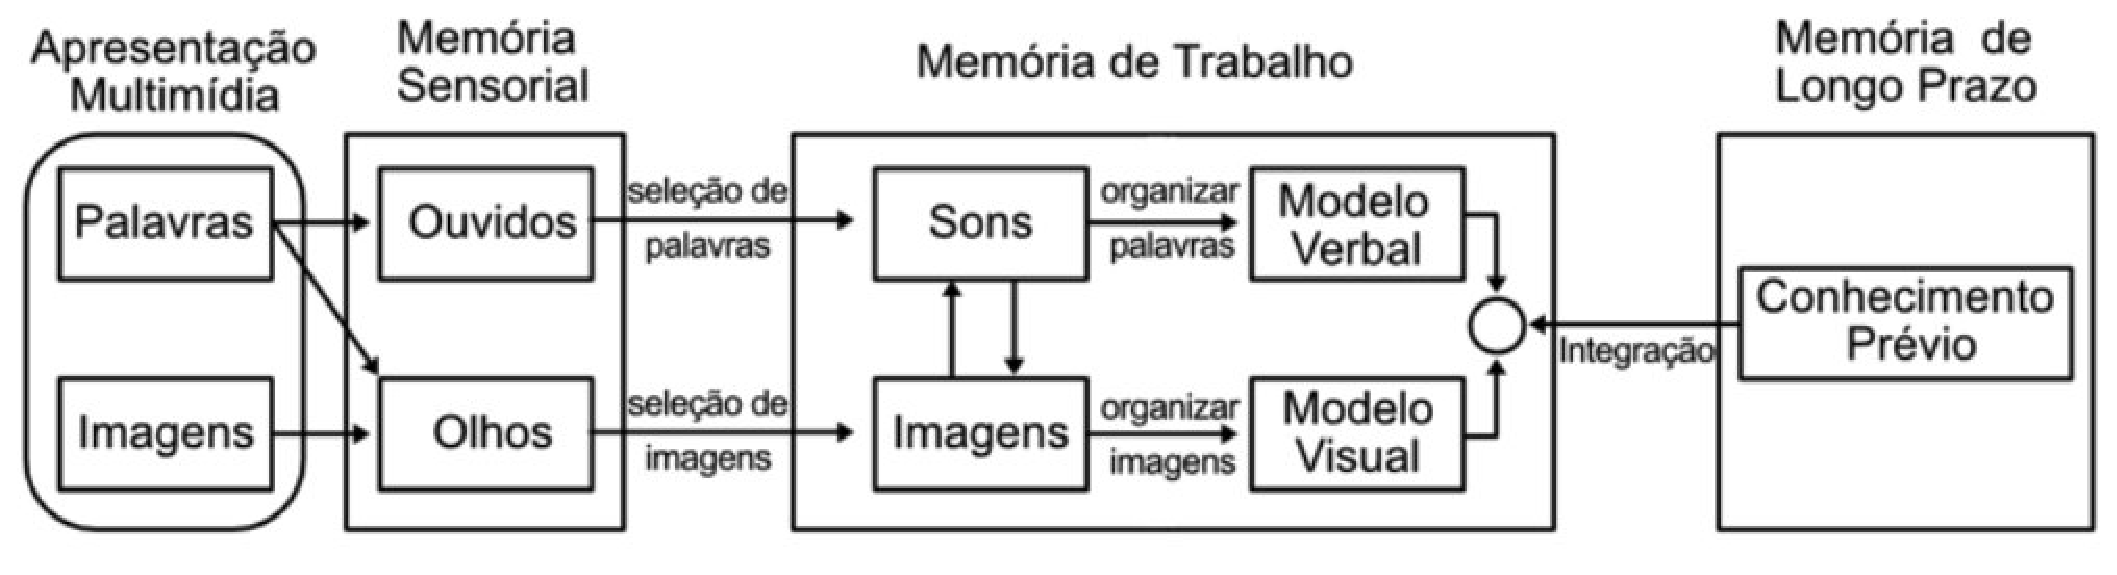
\includegraphics[width=.9\linewidth]{figuras/aprendizado.eps}
  	\caption{Teoria cognitiva para a aprendizagem multimídia}
  	\small{Fonte: \cite{mayer2001}}
  	\label{fig:aprendizado}
\end{figure}

Por tanto, para o desenvolvimento deste trabalho foram eleitos princípios consolidados pela teoria com o intuito de guiar a modelagem do sistema, princípios os quais: modalidade, redundância, diferenças individuais, segmentação e pré-treino \cite{clark2011, mayer2001, moreno2000}.

O princípio da modalidade indica que a aprendizagem é mais efetiva quando são utilizados recursos de video e narrativa ao invés de video e texto, isso se deve à forma que a memória de trabalho atua. Quando são apresentadas informações utilizando canais distintos, como visual e auditivo, a memória de trabalho possue melhor desempenho, pois não necessita manter as informações da mesma forma \cite{mayer2001}. 

O princípio da redundância complementa o anterior afirmando: O estudante aprende melhor com uso conjugado de recursos de video e narração do que recursos de video, texto e narração, se a informação visual for apresentada simultaneamente à narração. Porém, uma vez que as informações, visuais ou narrativas, são apresentadas de forma sequêncial, em geral a redundância levam à um melhor aproveitamento do que quando não existe a redundância \cite{moreno2000}.

O  princípio  das  diferenças  individuais  afirma  que  a  modelagem  do  material multimídia impacta muito mais o desempenho de estudantes de níveis inferiores do que o desempenho de estudantes mais avançados \cite{mayer2001}. Com base nesse princípio pode-se concluir que, o material educativo deve ser direcionado aos alunos de menores níveis.

O princípio da segmentação diz que ao dividir o conteúdo multimídia em partes menores a complexidado do material é relativamente menor, logo mais fácil de ser assimilada pelo aprendiz do que em um único material monolítico. A melhor assimilação do material é devido ao ajuste entre o fluxo de informação apresentada e o fluxo de informação absorvida pelo aluno \cite{mayer2001, moreno2000}.

O princípio do pré-treino determina que existe maior probabilidade de ocorrer aprendizagem significativa se o aluno conhecer os conceitos e tópicos antes da apresentação do material educativo \cite{mayer2001, moreno2000}.

\subsection{Vídeos interativos}

Videos interativos é um tema que está sendo pesquisado a mais de 30 anos e revela características promissoras desde os estudos iniciais, como por exemplo Gaudreau \textit{et al.} (1984) que realizou um estudo onde o objetivo era a construção de um \textit{Video Interactive Learning System} (VILS) na qual utilizou um video cassete e um monitor para tal feito \cite{gaudreau1984}.

Um estudo conduzido por Zhang (2005) mostrou que os estudantes que utilizaram o sistema proposto superou o desempenho dos estudantes que obtiveram aulas tradicionais. O sistema se tratava de um ambiente de aprendizagem virtual, onde o aluno tinha acesso a diversos tipos de mídias como slides, videos e animações. Zhang diz que o melhor desempenho do grupo que utilizou o sistema é possivelmente causado pela oportunidade de poder sempre questionar quando não compreendeu o que era ensinado ou repetir o video quantas vezes fosse necessário, o que normalmente não ocorre em aulas tradicionais, evidenciando a necessidade do aluno em adequar o ritmo em que as informação são apresentadas para evitar sobre carga cognitiva. O mesmo pode ser verificado em outros estudos mais recentes que mostram que quando o aprendiz controla do fluxo de informações o processo de aquisição de conhecimento pode ser mais rápido \cite{schwan2004, mayer2001}.

Assim a concepção do video interativo está fortemente ligada ao processo cognitivo do aprendiz, pois que dependendo da decisão tomada pelo aluno a cada ponto pode resultar em uma apredizagem significativa ou em falha \cite{moreno2000}. Videos interativos são compostos por fragmentos de videos conectados, acessados através de uma estrutura de decisão, existem dois modelos para a implementação: o modelo hipermidiático e o multimidiático \cite{wetzel1994}.

O modelo hipermidiático busca integrar elementos de hipertexto e hipermídias para o contexto dos videos interativos. Segundo o modelo, as ligações contidas nos videos interativos devem estar relacionadas temporalmente e até espacialmente aos conceitos de ancorágem. Por exemplo, no caso de um video que apresente conteúdo sobre teorias de aprendizagem, links sobre behaviorismo e cognitivismo devem aparecer possibilitando o aluno a adquirir a informação necessária no momento em que é apresentada, seja no mesmo video ou em outro video disponível \cite{wetzel1994}.

A priori este modelo pode parecer adequado, entretanto estudos atuais revelaram falhas que comprometiam a aprendizagem, pois acarretavam em sobrecarga cognitiva e atenção dividida, já que os alunos precisavam avaliar e escolher elementos que aparecia na tela e processar as informações extra \cite{zhang2005, moreno2000}.

Os princípios explorados por Mayer (2001) são heurísticas que se adequam ao modelo multimidiático e se mostram com boas soluções para problemas de sobrecarga cognitiva, atenção dividida entre outros explorados pelo pesquisador. Como exemplo de aplicação dessas heurísticas pode-se citar o agrupamento da informação visual e texto de forma espacial e temporalmente sincronizados quando necessário, o agrupamento de links para conteúdos possívelmente interessantes ao estudante ao final do video, a priorização da fala ao expor o conteúdo e apresentação geral do conteúdo antes de ser ministrado \cite{mayer2001}.

\section{Hipervídeos}

Hipervídeos são videos interativos que agregam características de hipermídias ou hiperdocumentos. Porém isto ainda é uma definição muito genérica do que são hipervídeos e existem algumas outras \cite{chambel2004}. Aubert \textit{et al.} (2005) enfatizam os benefícios de utilizar meta-dados de forma extrínseca ao documento audiovisual (DAV) por razões como por exemplo problemas na difusão do DAV por questões de licenças, ou ainda a possibilidade de diferentes pessoas poderem contribuir ou gerar novas informações de análise (meta-dados) sobre o DAV.

O potencial de aplicação de hipervídeos é vasto. Pesquisadores buscam integrar essa ferramenta em contextos como de filmes e documentários interativos, marketing, leitura de video ativa e aprendizagem. Em filmes e documentários interativos, é possivel ao espectador navegar pelos cenários, ou tomar outro caminho para a narrativa, aumentando assim a possibilidade do interessado encontrar um meio de assimilar melhor as informações apresentadas \cite{mozilla2012, sawhney1996, lippman1980, shipman2003}. De modo semelhante pode ser utilizado no marketing para demonstrar o uso de produtos e obter informações extras. Na área da aprendizagem pode ser utilizado como uma forma de prover ambientes de aprendizado rico no sentido de oferecer animações e facilitando a aprendizagem reflexiva e flexibilidade cognitiva \cite{zhan2004, shipman2003}.

\subsection{Principais características e componentes de sistemas de hipervídeos}

Sadallah \textit{et al.} (2012) destaca as principais características de sistemas de hipervídeos encontrados em sua pesquisa, sendo essas: interatividade, não-linearidade e enriquecimentos.

A interatividade dos hipervídeos está fundamentada na integração de espaços de hipermídias à videos, criando novas formas de interação e navegação de conteúdo através do espaço e do tempo, definidas na estrutura de hipermídias. A integração da estrutura de hipermídia possibilita que o usuário do sistema navegue de forma facilitada entre tópicos interessantes do próprio video ou até mesmo entre outros videos, permite a visualização estruturada dos videos e conteúdos.

Esse conceito pode ser melhor compreendido quando observa-se sistemas genéricos como o de anotações do Youtube, onde é possível relacionar videos em profundidade, ou HotVideo que generaliza o conceito de hiperlinks para textos e imagens permitindo a ligação entre o video digital e outros tipos de mídias \cite{sadallah2012, finke2004, faga2010}.

A não-linearidade está relacionada ao alto grau de flexibilidade que os hipervídeos agregam ao compor documentos baseados em video, estimulando a percepção do conhecimento ao promover uma leitura ativa que reflete no engajamento da audiência. Essa característica pode ser explorada através de montagens, inter-conexões e exibição sincronizada de videos diferentes \cite{sadallah2012}.

O enriquecimento do video inserido no hipervídeo pode ser feito de maneira externa. como por exemplo, pode ser apresentada uma tabela dos conteúdos que serão abordados no video, algum material posterior como imagens, textos, páginas da web ou outros tipos de elementos. O enriquecimento também pode acontecer no momento da reprodução do vídeo como links, sobreposição de gráficos ou figuras, legendas e títulos.

Sadallah \textit{et al.} (2012) afirma que com a evolução dos sistemas de hipervídeos, surgiram padrões de visualização e componentização. O estudo realiza uma análise dos componentes comuns à alguns sistemas de hipervídeos, sendo estes: Reprodutor de vídeo com controles, linha do tempo, sobreposição textual, sobreposição de gráficos, pontos de ligação, tabela de conteúdos, mapa do vídeo, transcrição.

\begin{itemize}
	\item Reprodutor de vídeo com controles - Esse componente é comum entre todos os sistemas.
	\item Linha do tempo - É o componente que integra uma visão espacial da dimensão temporal dos meta-dados no vídeo e permite o usuário navegar diretamente por ele para outras posições temporais da reprodução.
	\item Sobreposição textual - Apresenta textos sobrepostos ao vídeo.
	\item Sobreposição de gráficos - Apresenta gráficos como imagens sobrepostos ao vídeo.
	\item Pontos de ligação - Consiste em uma sobreposição gráfica que haje como hiperlinks.
	\item Tabela de conteúdos - É uma representação textual do conteúdo do vídeo.
	\item Mapa do vídeo - Se comporta como uma tabela de conteúdos com uma representação gráfica dos meta-dados.
	\item Transcrição - É o texto gerado a partir da transcrição do conteúdo audiovisual.
\end{itemize} 

\subsection{Hipervídeos orientado à anotações}

Vídeos são tipos de dados que, intrínsicamente, não permitem acesso convencional aos dados, busca ou indíces para organização de fragmentos. Partindo disso, surgiram questionamentos sobre como navegar entre partes precisas do vídeo, enriquecer, reorganizar e explicar o conteúdo. Esses questionamentos levaram a soluções como o uso de anotações \cite{sadallah2012}.

Aubert \textit{et al.} (2005) definem um documento audiovisual anotado (DAA) como sendo um DAV associado à meta-dados com estrutura de anotação (EA) que possue relação espaço-temporal com o documento, fragmentos do video e possívelmente com os próprios elementos da EA. Logo, a visualização de um DAA pode ser definida como um modo de visualizar as informações do DAA utilizando as informações contidas na estrutura de anotação em conjunto com o documento audiovisual.

Isso pode ser melhor entendido observando a figura \ref{fig:diagram_DAVOA} que mostra o \textit{Advene}, sistema propósto por Aubert e Prié em 2005. Partindo destes conceitos será adotada para este trabalho a definição de hipervídeo como sendo uma visualização do documento audiovisual anotado com estrutura de anotação com possibilidade de controlar a reprodução (temporalidade) \cite{aubert2005}.

\begin{figure}[h!]
	\centering
  	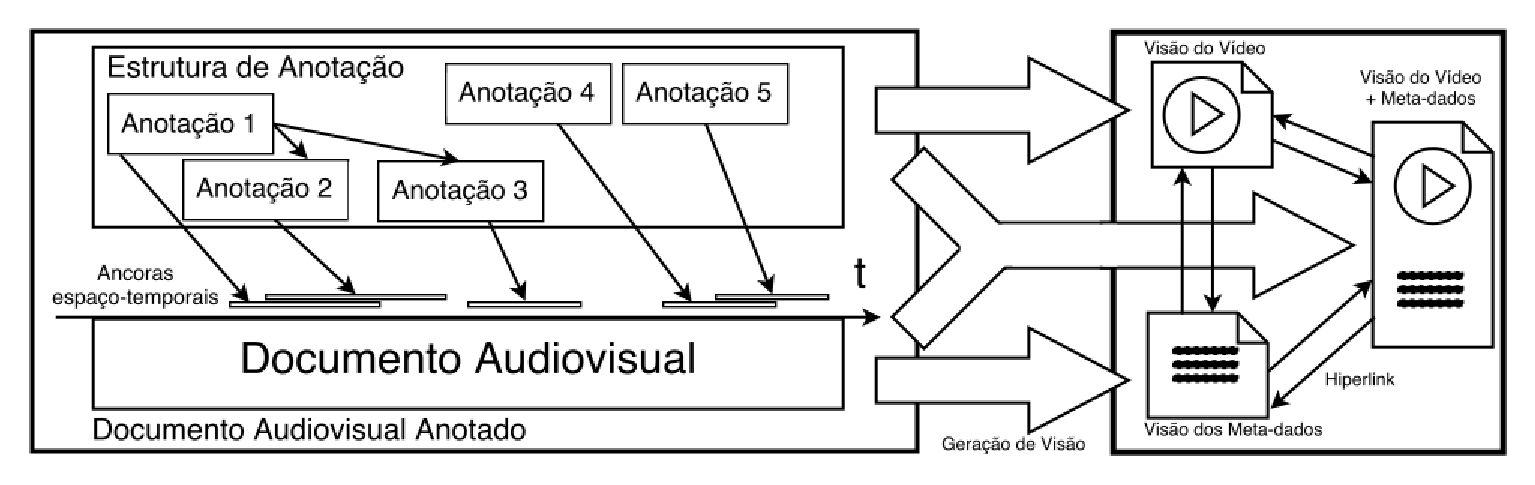
\includegraphics[width=.9\linewidth]{figuras/diagram_DAVOA.eps}
  	\caption{Representação de um hipervídeo orientado à anotações.}
  	\small{Fonte: \cite{sadallah2012}}
  	\label{fig:diagram_DAVOA}
\end{figure}

Com a utilização das anotações surgem novas maneiras de fazer uso de vídeos, podendo então quebrar a lineridade, enriquecer o conteúdo e prover interatividade do vídeo. Sadallah \textit{et al.} (2012) cita vários sistemas de hipervídeos e afirma que a maioria utiliza sistemas de anotações, porém as soluções ainda são muito acompladas aos videos, quando não são completamente integradas ao reprodutor. Esse tipo de soluções não contribuem para o estabelecimento de um padrão de desenvolvimento de hipervídeos, por outro lado soluções como o \textit{Advene} (Aubert \textit{et al.} 2005) propõe um modelo menos acoplado, passível de evolução.

As anotações podem ser geradas de forma semi-manual, onde uma pessoa gera as informações de análise em uma camada superior ao vídeo com o uso de softwares para tal, ou automátizada no caso dos dados serem gerados pelo software de análise de forma independente do julgamento humano. Esses modos de gerar as anotações possuem suas vantagens e desvantagens, por exemplo na forma semi-manual, as anotações tendem a ser mais precisas e melhor elaboradas. Por outro lado, com o uso de softwares que automatizam o processo de criar anotações se torna mais rápido e menos custoso. Ainda existe a possibilidade de gerar meta-dados de análise de forma completamente manual, sendo esta porém a forma mais custosa de criar anotações \cite{sadallah2012}.

\section{Engenharia de Software}

Devido à alta complexidade intrínseca ao desenvolvimento de sistemas de software, se faz necessária a aplicação de técnicas de engenharia voltadas para a resolução de problemas, como por exemplo de levantamento de requisitos, manutenção e evolução do software, testes e qualidade. 

Schach (2009) apresenta dados sobre o estado final de 9.236 projetos de software até o ano de 2004. Segundo esse autor apenas 29\% dos projetos foram concluídos com sucesso, ao passo que 18\% foram cancelados e 53\% foram concluídos porém com atraso, orçamento excedido ou com menos funcionalidades que o previsto.

A engenharia de software é definida como uma disciplina cujo objetivo é a produção de sistemas softwares isento de falhas, entregue no prazo e orçamento definido e atenda as necessidades do cliente. Um dos primeiros pesquisadores a falar sobre engenharia de software é  Boehm em 1976. Ele cita diversas práticas utilizadas na época, porém algumas coisa mudaram na engenharia de software desde então \cite{schach2009, boehm1976}.

A utilização de metodologia ágil de desenvolvimento é uma tendência atual e crescente no contexto da engenharia de software, assim como o uso de ferramentas de integração, gerência de configuração e automatização de testes. Nas seções a seguir serão abordados os tópicos de metodologias ágeis, arquitetura de software, testes e reutilização de software.

\subsection{Metodologia Ágil}

Métodos ágeis são práticas de desenvolvimento de software de forma enxuta que surge em oposição aos métodos tradicionais, considerados rigorosos e burocráticos. O termo métodos ágeis foi cunhado por 17 especialistas que buscavam meios mais rápidos, leves e centrados à pessoas de desenvolver software, criando assim o manifesto ágil composto pelos seguintes valores.

Valores das metodologias ágeis:
\begin{itemize}
	\item Indivíduos e interação mais que processos e ferramentas.
	\item Software funcionando mais que documentação abrangente.
	\item Colaboração com o cliente mais que negociação de contratos.
	\item Responder à mudanças mais que seguir um plano.
\end{itemize}

Os métodos ágeis são implementados por diversos modelos de trabalho (\textit{frameworks}) como o scrum, xp e crystal, entre outros. Esses frameworks definem práticas de acordo com os valores e princípios ágeis, buscando uma maior eficiência ao lidar com projetos de até certo grau de complexidade \cite{prik2014}.

O scrum é baseado no empirismo sendo um dos mais populares no contexto da engenharia de software. Este framework possui três pilares fundamentais: transparência, inspeção e adaptação. A transparência consiste em possibilitar que os interessados conheçam claramente o resultado das atividades, erros do projetos entre outras características importantes do projeto como os termos utilizados e a definição deles. A inspeção visa identificar problemas nos artefatos produzidos servindo de insumo para tomadas de decisões necessárias para que haja mudanças. A adaptação acontece quando problemas inaceitáveis ocorrem \cite{scrum2014}.

Algumas práticas do scrum serão adotadas neste trabalho, por tanto é necessário compreender melhor os conceitos envolvidos neste processo.

\begin{itemize}
	\item Product Owner (P.O.): Dono do produto, aquele que define o que será desenvolvido (\textit{backlog}) e o que tem valor no produto entregue.
	\item Scrum master: Atua em conjunto com o P.O. para definir o backlog, além de organizar, motivar a equipe e facilitar o desenvolvimento removendo qualquer empecilho.
	\item Equipe de desenvolvimento: A equipe de desenvolvimento do software.
	\item Sprint: O período de tempo em que deve ser realizado o trabalho definido.
\end{itemize}

Além desses conceitos existem também os eventos de revisão da sprint, quando é averiguado em conjunto com o cliente o que foi realizado na sprint; planejamento da sprint, quando é definido o pacote de trabalho da sprint; e a retrospectiva, quando o trabalho que foi desempenhado pelo time scrum é analisado internamente pelo próprio time \cite{prik2014}. Os conceitos abordados anteriormente podem ser melhor observados na figura \ref{fig:scrum}. No contexto deste trabalho, o backlog consiste nas necessidades levantadas para a elaboração deste sistema; o product owner se trata do orientador; a equipe de desenvolvimento sendo o autor.

\begin{figure}[h!]
	\centering
  	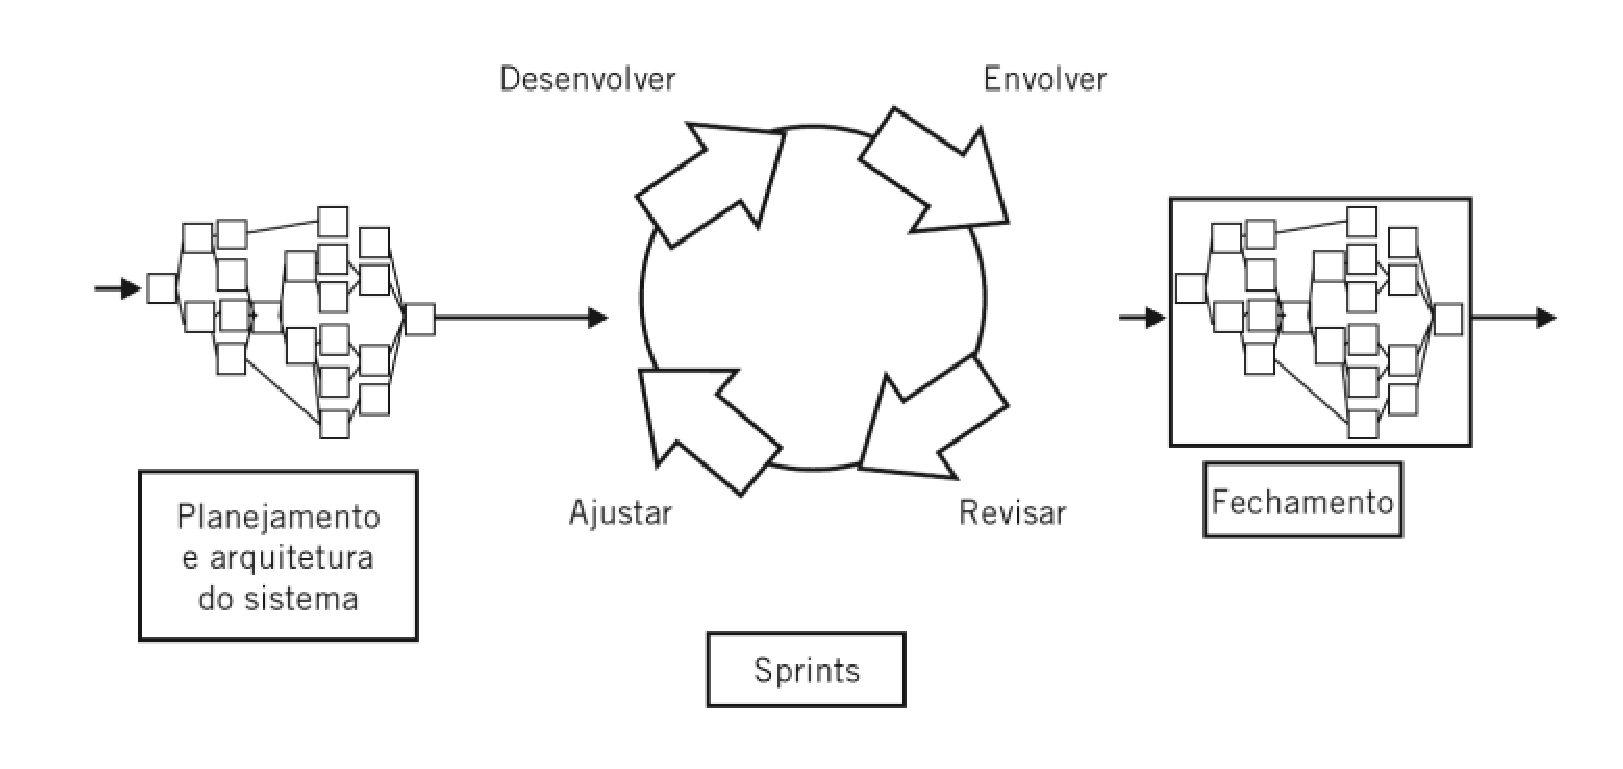
\includegraphics[width=.9\linewidth]{figuras/scrum.eps}
  	\caption{Representação do processo scrum.}
  	\small{Fonte: \cite{scrum2014}}
  	\label{fig:scrum}
\end{figure}

\subsection{Arquitetura de Software}

Arquitetura de software é um conjunto de descisões da organização do sistema de software, das interfaces de comunicação e dos elementos estruturais que suportarão os componentes com relação ao comportamento e funcionalidades pretendidas para o sistema. Esta organização segue um estilo arquitetural que guia a evolução das estruturas de subsistemas de modo a compor todo o sistema. Neste trabalho o estilo arquitural adotado é o \textit{Model-View-Controller} (MVC) \cite{clements2010}.



\subsection{Testes}

\subsection{Reutilização de Software}

